\documentclass[sigconf]{acmart}

\usepackage{graphicx}
\usepackage{algorithm} % for algorithms
\usepackage{algpseudocode}
\usepackage{booktabs} % For formal tables
\usepackage{amsthm} % For claims
\usepackage{bbm} % indicator function

% table
\usepackage[flushleft]{threeparttable} % http://ctan.org/pkg/threeparttable
\usepackage{booktabs,caption}

\theoremstyle{remark}

\settopmatter{printacmref=true, printccs=true, printfolios=true}
\pagestyle{empty} % removes running headers

\newcommand{\PicScale}{0.5}
\newcommand {\FlameStream} {FlameStream}
\begin{document}

% \copyrightyear{2019} 
% \acmYear{2019} 
% \acmConference[BIRTE 2019]{Real-Time Business Intelligence and Analytics}{August 26, 2019}{Los Angeles, CA, USA}
% \acmBooktitle{Real-Time Business Intelligence and Analytics (BIRTE 2019), August 26, 2019, Los Angeles, CA, USA}
% \acmPrice{15.00}
% \acmDOI{10.1145/3350489.3350491}
% \acmISBN{978-1-4503-7660-0/19/08}

\title {Distributed Change Detection in Data Sreams}

\author{Mikhail Yutman}
\affiliation{%
  \institution{Yandex}
  \city{Saint Petersburg}
  \country{Russia}}
\email{myutman@yandex-team.ru}

\author{Artem Trofimov}
\affiliation{%
  \institution{Yandex}
  \city{Saint Petersburg}
  \country{Russia}}
\email{tomato@yandex-team.ru}

\author{Igor Kuralenok}
\affiliation{%
  \institution{Yandex}
  \city{Saint Petersburg}
  \country{Russia}}
\email{solar@yandex-team.ru}

\author{Boris Novikov}
\affiliation{%
  \institution{National Research University Higher School of Economics}
  \city{Saint Petersburg}
  \country{Russia}}
\email{borisnov@acm.org}

\begin{abstract}

% High-frequent stream processing is a very important research area. Powerful streaming algorithms are widely used in banking and financial analytics as the data is too huge to store it and also arrives at high frequencies so it needed to be processed as soon as possible to make a timely decision. Change-point detection on a streaming data is used to track changes in credit card transactions, stock market ticks or computer network traffic. By the way, data can be produced too frequent, so it's desirable to distribute change-point detection over multiple nodes. Also values of statistics can be dependent and it's a challenge. In this paper we introduce a distributed stream processing algorithm for change-point detection and try to explore importance of dependencies between incoming statistics.

Change detection algorithms are widely used in data flows that monitor suspicious activity in credit card transactions, stock market ticks, or computer network traffic. Another application is to track unexpected fluctuations in data used for training online machine learning models. To make these data flows scalable, it is natural to run them on distributed stream processing systems such as Flink, Storm, Spark Streaming, etc. Usually, we don't have an information about probability distribution of data. However, change detection algorithms either aim to a case when all data stream items are handled by a single worker or require an information about probability distribution of data. In this work, I complement an existing efficient change detection algorithm that doesn't need information about probability distribution of data to be suitable for a distributed stream processing engine. However, scalability has its price. Experiments demonstrated an emerging trade-off between scalability together with false alarm probability on the one side, and change detection accuracy together with detection latency on the other side.

% To  By the way, data can be produced too frequent, so it's desirable to distribute change-point detection over multiple nodes. Also values of statistics can be dependent and it's a challenge. In this paper we introduce a distributed stream processing algorithm for change-point detection and try to explore importance of dependencies between incoming statistics.

\end{abstract}

\maketitle

\thispagestyle{empty}

\section {Introduction}
\label {fs-acker-intro}

%State-of-the-art distributed stream processing systems such as Flink~\cite{Carbone:2017:SMA:3137765.3137777}, Heron~\cite{Kulkarni:2015:THS:2723372.2742788}, or MillWheel~\cite{Akidau:2013:MFS:2536222.2536229} are able to execute complex dataflows consisted of multiple operators that can be partitioned among workers. Each operator may execute almost arbitrary user-defined code which transforms elements into other ones or filters them out. After multiple transformations, it may be not clear which ingested by a system input element spawned an output record. 



To satisfy {\em consistency} and {\em fault tolerance} requirements, modern streaming engines support {\em dependency tracking} between input and output elements. Tracking mechanisms usually provide notifications that some set of ingested elements has already been transformed into outputs by the whole dataflow or its part. Such notifications are required for a plenty of problems: consistent {\bf state snapshotting}~\cite{Akidau:2013:MFS:2536222.2536229, 2015arXiv150608603C} to provide for correct failure-recovery, {\bf transactional processing} to ensure {\em delivery guarantees}~\cite{thepaper, Carbone:2017:SMA:3137765.3137777}, {\bf data producer cleanup}~\cite{Noghabi:2017:SSS:3137765.3137770} to support recovery while persistently storing only a part of input records, and so on. 

Although most of the mentioned problems have been extensively studied for databases~\cite{DBLP:books/mk/WeikumV2002}, classical databases do not commonly face the problem of matching input and output because they mostly work with fixed input data. Therefore, for instance, transactional processing methods employed in databases cannot be used as-is in streaming systems without an adaptation of some dependency tracking technique.

Most streaming systems apply one of the following approaches for dependency tracking: {\em micro-batching} and {\em markers}. In micro-batching, the output element may be originated only by an input one from the same micro-batch. Therefore, the completeness of a micro-batch indicates that all input elements within this batch are transformed into output elements. Markers approach bases on an injection of special input elements into a dataflow. These elements are broadcasted to each partition of the next operator and play the role of separators between ordinary records. Receiving such element from all partitions indicates that all operators up to the stream have entirely processed a particular set of input elements. 

Both micro-batching and marker approaches have limitations and can induce high overhead on regular processing. Micro-batching has well-known issues with latency-conscious dataflows~\cite{S7530084}. Besides, it is hard to track individual records due to the ineffectiveness of very small micro-batches~\cite{Zaharia:2012:DSE:2342763.2342773}. The application of marker-based methods is limited for cyclic dataflows~\cite{Carbone:2017:SMA:3137765.3137777}. Besides, as we show further, markers may induce significant overhead on throughput due to a huge amount of extra network traffic.

In this work, we present~\tracker , a dependency tracking technique that provides for individual elements monitoring, while inducing a small overhead on regular processing. On the one hand, \tracker\ is suitable for a fair element-at-time streaming model without the need of micro-batching. On the other hand, it supports cyclic dataflows and requires a small amount of service traffic. \tracker\ can also monitor streaming elements within parts of dataflow as well as marker-based techniques. \tracker\ is deployed as an external agent that can scale out to sustain a high rate of input records. 

This paper extends preliminary publications~\cite{we2018beyondmr, we2018adbis, thepaper}, which describe a stream processing system that uses~\tracker\ as a component. In this paper, we detail a formal concept of~\tracker , propose its distributed implementation, and evaluate the~\tracker\ performance in a more narrowly focused way. Our main contributions are:
\begin{itemize}
    \item Design of general formal concepts for a dependency tracking mechanism
    \item Transformation of these concepts into the~\tracker\ using ideas from Apache Storm {\em \acker}~\cite{Toshniwal:2014:STO:2588555.2595641}
    \item Centralized and distributed implementations which are suitable for cyclic dataflows
    \item Demonstration of the \tracker\ practical feasibility and performance insights
\end{itemize}

The rest of the paper is organized as follows: Section~\ref{fs-acker-motivation} gives an overview of existing dependency tracking solutions and practical tasks that require a tracking mechanism. In Section~\ref{fs-acker-design}, we design formal concepts for dependency tracking methods and turn these concepts into the \tracker\ mechanism. Section~\ref{fs-acker-impl} summarizes the implementation of \tracker\ for both centralized and distributed setups with optimizations that can reduce the amount of extra traffic. In Section~\ref{fs-acker-related}, we show that the proposed technique is scalable, and can outperform alternatives employed in state-of-the-art stream processing engines. Finally, we discuss related work and our conclusions in Section~\ref{fs-acker-related} and Section~\ref{fs-acker-conclusion}, respectively.

\section {Motivation}
Most change-point detection algorithms are not intended for usage in distributed mode. Experimentally obtained results show that algorithm used in single-node mode can really slow the stream processing graph.

\begin{figure}[h]
    \centering
    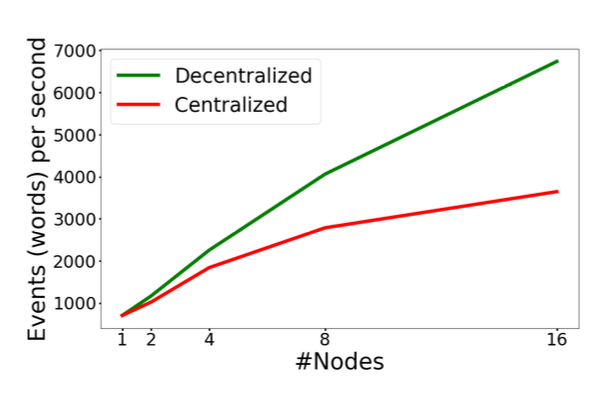
\includegraphics[scale=0.7]{throughput.png}
\end{figure}

``Decentralized'' line depicts throughput of system with distributed algorithm of change-detection while ``Centralized'' corresponds to throughput of system with single-node algorithm.

Thus, development an efficient distributed change-point detection algorithm is a practically important problem.

\section {Method}
\subsection{Single-node algorithm}

Single-node algorithm should process elements from stream and return a statistic that characterises a state of the substream that was processed by this node.

We use the window technique from the paper \cite{kifer2004detecting} which involves two windows. The first window, called reference, stands at the beginning of the stream and another one, called sliding, moves as soon as a new element arrives.

After each processed element we calculate the distance between the samples that refer to reference and the sliding windows respectively, which we denote as $s_t$. We use the Kolmogorov-Smirnov statistic as a distance function between two samples. To be more precise we calculate the statistic from Kolmogorov-Smirnov test for empirical distributions of two samples which is $$KS(X, Y) = \max_x \left|F_X(x) - F_Y(x)\right|$$ for samples $X$ and $Y$ with emperical distributions $F_X$ and $F_Y$ respectively.

We can use $s_t$ itself as a statistic for this node, but it's very local and doesn't anything about the data processed before. We can also use maximum among all the statistics as it was suggested in \cite{kifer2004detecting}, but maximum doesn't actually contain full information about processed substream and can be very sensible to outliers.

We suggest an approach that involes smoothing of statistic by adding older statistic to current one with the lower weight. More precisely we propose to calculate the following values: $$n_t := 1 + \lambda n_{t - 1} $$ $$S_t := s_t + \lambda S_{t - 1}$$ $$\hat{s}_t := S_t / n_t$$ and use the value $\hat{s}_t$ as a statistic from the node. We assume that such a statistic can decrease the level of false detections with the same detection quality because it's more outlier resistant as far as it takes previous values into account.

% More precisely we calculate the following statistic and return it as a result fo this node $$S_t = \max_{1 \le i \le t - (n + m) + 1} KS(reference, sliding_i)$$, where  is Kolmogorov-Smirnov statistic for emperical distributions $F_X$ and $F_Y$ of samples $X$ and $Y$.

\subsection{Fusion rule}

Fusion rule should recieve statistics from different nodes and decide wheter change has already happened or not.

We apply a simple multivariable function such as maximum, median or mean. We compare the obtained value to the precomputed threshold and if it's greater than change is thought to be having occurred.

\section {Experiments}
\label {fs-lightbulbs-experiments}

    
\begin{table}[h]
    \centering
    \begin{tabular}{|l||l|l|l|l|}
        \hline
         & KS & KSI & $\phi$ & $\Xi$ \\ \hline
        baseline & 8 & 9.8 & 3.6 & 7.2 \\ \hline
        1 node & 1.8 & 3.4 & 6.4 & 7.8 \\ \hline
        4 nodes & 6.2 & 7.2 & 16.8 & 14.0 \\ \hline
        8 nodes & 8.6 & 9.4 & 16.4 & 14.2 \\ \hline
        16 nodes & 13.0 & 15.0 & 14.0 & 18.4 \\ \hline
    \end{tabular}
    \caption{Experiment without changes. False detections}
\end{table}

\begin{table}[h]
    \centering
    \begin{tabular}{|l||l|l|l|l|}
        \hline
         & KS & KSI & $\phi$ & $\Xi$ \\ \hline
        baseline & 31 & 60 & 92 & 86 \\ \hline
        1 node & 27.4 & 53.8 & 75.0 & 67.6 \\ \hline
        4 nodes & 31.8 & 60.4 & 71.6 & 66.4 \\ \hline
        8 nodes & 25.2 & 60.0 & 67.0 & 61.8 \\ \hline
        16 nodes & 19.4 & 47.8 & 53.0 & 50.6 \\ \hline
    \end{tabular}
    \caption{Experiment 1. True detections}
\end{table}



\begin{table}[h]
    \centering
    \begin{tabular}{|l||l|l|l|l|}
        \hline
         & KS & KSI & $\phi$ & $\Xi$ \\ \hline
        baseline & 30 & 34 & 20 & 19 \\ \hline
        1 node & 25.2 & 25.8 & 21.8 & 23.8 \\ \hline
        4 nodes & 26.2 & 24.0 & 20.4 & 19.0 \\ \hline
        8 nodes & 27.4 & 22.2 & 17.4 & 19.0 \\ \hline
        16 nodes & 25.8 & 22.0 & 21.4 & 22.8 \\ \hline
    \end{tabular}
    \caption{Experiment 1. Errored detections (false and late)}
\end{table}

\begin{table}[h]
    \centering
    \begin{tabular}{|l||l|l|l|l|}
        \hline
         & KS & KSI & $\phi$ & $\Xi$ \\ \hline
        baseline & 0 & 4 & 16 & 13 \\ \hline
        1 node & 0.8 & 5.4 & 9.8 & 3.4 \\ \hline
        4 nodes & 3.2 & 11.2 & 12.2 & 9.8 \\ \hline
        8 nodes & 2.8 & 10.6 & 12.2 & 10.4 \\ \hline
        16 nodes & 1.4 & 5.8 & 10.8 & 8.4 \\ \hline
    \end{tabular}
    \caption{Experiment 2. True detections}
\end{table}

\begin{table}[h]
    \centering
    \begin{tabular}{|l||l|l|l|l|}
        \hline
         & KS & KSI & $\phi$ & $\Xi$ \\ \hline
        baseline & 15 & 32 & 33 & 36 \\ \hline
        1 node & 8.2 & 22.8 & 23.2 & 18.4  \\ \hline
        4 nodes & 11.6 & 25.0 & 25.6 & 20.4 \\ \hline
        8 nodes & 15.8 & 23.6 & 24.6 & 24.6  \\ \hline
        16 nodes & 13.4 & 27.6 & 27.0 & 24.4 \\ \hline
    \end{tabular}
    \caption{Experiment 2. Errored detections (false and late)}
\end{table}




% \section {Screaming challenges}
% \label {fs-solution}

\subsection{Reproducibility and Fault Tolerance}

{\em Exactly-once} and determinism are desirable properties for the text classification data flow. On the other hand, one of the key performance metrics in streaming applications is latency. Table~\ref{comparison} shows if a system supports exactly-once, built-in determinism, and low latency (less than 500 ms). To the best of our knowledge, among open systems only~\FlameStream\ provides for both low latency, determinism, and exactly-once. This property is achieved using optimistic total order enforcement. The details of this approach are discussed in~\cite{we2018adbis, we2018beyondmr}. Implementation of the text classification data flow on top of~\FlameStream\ can potentially resolve the trade-offs between reliability and performance.

\begin{table}[htbp]
\caption{Comparison of stream processing systems}
\begin{threeparttable}
\begin{tabular}{lccc}
System & Exactly-once & Determinism & Latency    \\
\hline
Storm, Heron, Samza  &    --      &   --       &   low            \\
Spark Streaming    &    +       &   +        &   high           \\
Flink              &    +       &   -        &   high$^*$       \\
MillWheel          &    +       &   +        &   NA             \\
FlameStream        &    +       &   +        &   low            \\
\end{tabular}
* with enabled {\em exactly-once}~\cite{we2018beyondmr}
\end{threeparttable}
\label{comparison}
\end{table}

\subsection{Concept Drift}

Streaming applications often experience {\em concept drift}: the statistical properties of the target, which the machine learning model is trying to predict, change over time. Regarding news articles classification, concept drift may lead to the following effects:

\begin{itemize}
    \item Meaning of some terms is changing over time. For example, word {\em goal} in the article published during the soccer world cup is most likely related to soccer. On the other hand, during the world hockey cup, it rather belongs to the hockey topic.
    \item News topic may appear and vanish over time. For example, some important events can transform into a separate news topic for a time as it happens with large political or sports forums. However, after some time such topics can disappear form a news agenda.
\end{itemize}

A streaming classifier must handle such behavior to automatically fit in rapidly changing news data. We propose a modification of the data flow for prediction with online training that aims to handle concept drift. Training is a separate branch within the logical graph presented in section~\ref{fs-framework}. The modified data flow is shown in Figure~\ref{training_graph}. Assume that the input stream consists of two types of elements: pre-labeled and raw. The latter elements must be labeled by a classifier and delivered to end-user. For already labeled text its features are sent to a {\em Partial fit} vertex instead of the {\em Classifier}. {\em Partial fit} vertex updates machine learning model and sends it to {\em Text Classifier} vertice.

\begin{figure}[htbp]
  \centering
  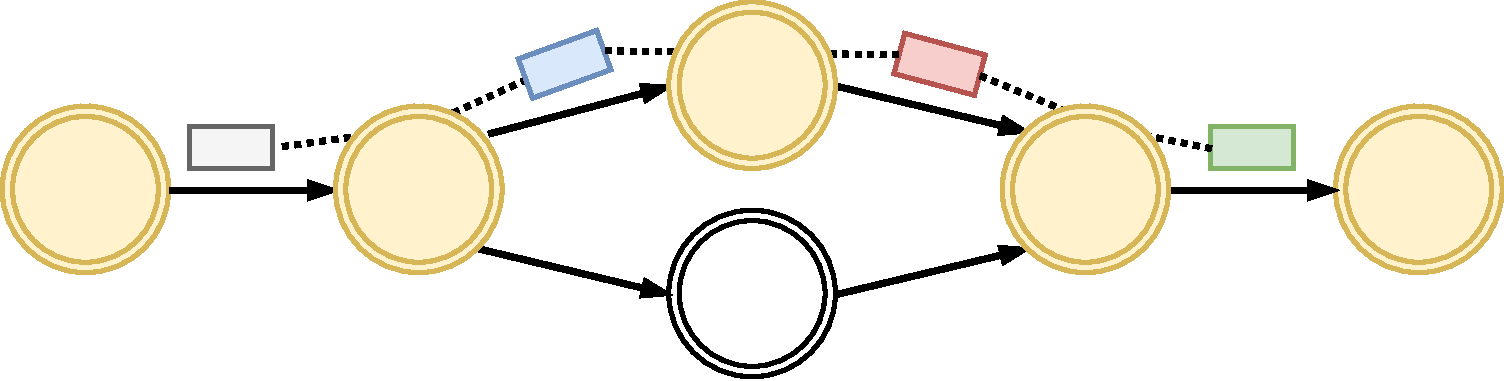
\includegraphics[scale=0.32]{pics/logical-graph}
  \caption{Data flow with online training}
  \label {training_graph}
\end{figure}

A potential issue is that the training process may be time-consuming. If training and prediction processes run consecutively, there will be significant latency spikes, e.g. if a training process lasts for several minutes, then spikes can be thousands times greater than the latency for prediction. However, without synchronization, there will be no reproducible correspondence between texts and applied model. It is almost impossible to achieve the same results within a new run on the same data because the training time becomes a hidden parameter that influences output. 

For instance, assume that we make two runs. On the first run model update takes 70 seconds, but on the second run 75 seconds due to extra CPU load. If training and predicting are not synchronized, more unlabeled input elements are processed by an outdated model in the second case so the distribution of news topics may be different between these two runs. To solve this issue, we propose using efficient online learning algorithms, e.g. FTRL proximal~\cite{mcmahan2013ad}. In this case, model updating is smooth and its synchronization with training does not cause latency spikes.

% \section{Related Work}
% 

Most related prior works were implemented on Apache Spark \cite{semberecki2016distributed} \cite{8029336} \cite{Nodarakis2016LargeSS} \cite{baltas2016apache} \cite{svyatkovskiy2016large} or Apache Storm \cite{khumoyun2016real}. These platforms use micro-batching technique for processing data. However, such method provides high latency between obtaining a text and labelling it. In addition, all the methods above does not consider a concept drift as an issue.

Next work takes into account the concept drift and related to stream data nature \cite{zhang2008one}. However, the final solution is hard to scale into a cluster of machines efficiently.

\section{Conclusion and Future Work}
\label {fs-lightbulbs-conclusion}

%In this work, we formulated and formalized a problem of dependency tracking between input and output elements in streaming dataflows. We demonstrated that state-of-the-art distributed stream processing systems face this problem in state snapshotting mechanisms~\cite{Carbone:2017:SMA:3137765.3137777, apache:storm}, the materialization of time-varying relations~\cite{Begoli:2019:OSR:3299869.3314040}, and atomic delivery of all descendants of an input item~\cite{we2018adbis}.  
In this paper we formulated and formalized a problem of distributed change-point detection in streaming dataflows. We analysed the importance of dependencies in data distribution over nodes and intoduced our version of algorithm for distributed change-point detection.

%To solve this problem, we proposed a mechanism that adopts ideas from the Apache Storm completion tracking mechanism called \acker. We extend each data item with a logical timestamp that denotes corresponding input items and track if dataflow contains elements with specific timestamps. Our solution, called \tracker, provides the following features:
%\begin{itemize}
%    \item {\bf Fine-grained tracking:} \tracker\ efficiently watches and provides notifications that system completely processed some set of input items even for individual input elements.
%    \item {\bf Cyclic graphs support:} proposed mechanism works for cyclic execution graphs, and that makes it suitable for iterative dataflows as well. 
%    \item {\bf Scalability:} we introduced a decentralized version of \tracker\ that allows a system to distribute extra network traffic between all computational units. 
%    \item {\bf Low overhead:} \tracker\ does not produce any significant performance penalty and does not affect the throughput of a distributed streaming dataflow.
%\end{itemize}

%We conducted a series of experiments and compared the proposed method with a baseline approach based on the checkpointing mechanism used in Apache Flink. We demonstrated that both centralized and decentralized implementations of \tracker\ provide lower notification latency that does not considerably degrade with an increase of a logical graph size or a cluster size. Experiments also showed that \tracker\ has lower throughput overhead in case of fine-grained tracking.

We conducted a series of experiments and compared the proposed method with a single-node methods and demonstrated that it keeps acceptable values of metrics and provides lower latency.

\bibliographystyle{ACM-Reference-Format}
\bibliography{bibliography/flame-stream}

\end {document}

\endinput
